\section{An\'alisis}

\subsection{La Universidad Rusa de la Amistad de los Pueblos (URAP)}
Vamos a realizar un an\'alisis de nuestro traceroute sobre "La Universidad Rusa de la Amistad de los Pueblos (URAP)". Es una universidad que se encuentra en Rusia, en la ciudad de Mosc\'u.\newline

El host de dicha universidad es http://www.rudn.ru/ (IP: 193.232.218.50).\\	

\subsubsection{Par\'ametros de entrada}
\begin{itemize}
\item Host: www.rudn.ru
\item Tiempo Limite: 2
\item Cant. Iteraciones en cada nodo: 10
\item Recorrido m\'aximo de nodos: 30 (TTL m\'aximo)
\item alpha: 0.05
\end{itemize}
El tiempo limite indica cuanto esperar de respuesta, como m\'aximo, a un nodo.\newline

\subsubsection{Resultados obtenidos}

Captura general de los resultados obtenidos:

TTL:  1    IP Source: 192.168.43.1       Argentina - Buenos Aires - Capital Federal\\
TTL:  2    IP Source: 172.21.216.35      Argentina - Buenos Aires - Capital Federal\\
TTL:  3    IP Source: 172.21.216.49      Argentina - Buenos Aires - Capital Federal\\
TTL:  4    IP Source: 172.21.220.98      Argentina - Buenos Aires - Capital Federal\\
TTL:  5    IP Source: 172.21.220.98      Argentina - Buenos Aires - Capital Federal\\
TTL:  6    Obtuvimos time out, dado que el nodo 6 no contesto. \\
TTL:  7    IP Source: 172.21.224.114     Argentina - Buenos Aires - Capital Federal\\
TTL:  8    IP Source: 172.21.224.114     Argentina - Buenos Aires - Capital Federal\\
TTL:  9    IP Source: 172.21.224.113     Argentina - Buenos Aires - Capital Federal\\
TTL: 10    IP Source: 172.16.1.5         Argentina - Buenos Aires - Capital Federal\\
TTL: 11    IP Source: 181.88.80.213      Argentina - Entre Rios - Federal\\
TTL: 12    IP Source: 190.225.252.162    Argentina - Entre Rios - Federal\\
TTL: 13    IP Source: 195.22.220.53      Argentina - Buenos Aires - Tigre\\
TTL: 14    IP Source: 89.221.41.175      Italia\\
TTL: 15    IP Source: 89.221.41.175      Italia \\
TTL: 16    IP Source: 80.239.193.161     Suiza\\
TTL: 17    IP Source: 62.115.141.125     Suiza\\
TTL: 18    IP Source: 80.91.245.99       Suiza\\
TTL: 19    IP Source: 213.248.64.33      Suiza \\
TTL: 20    IP Source: 62.115.139.172     Suiza \\
TTL: 21    IP Source: 80.91.250.96       Suiza\\
TTL: 22    IP Source: 62.115.42.38       Suiza\\
TTL: 23    IP Source: 194.85.40.229      Rusia - San Petersburgo\\
TTL: 24    IP Source: 194.85.40.214      Rusia - San Petersburgo\\
TTL: 25    IP Source: 194.190.255.42     Rusia - San Petersburgo \\
TTL: 26    IP Source: 193.232.212.99     Rusia - Moscu\\
TTL: 27    Obtuvimos time out, dado que el nodo 27 no contesto. \\
TTL: 28    IP Source: 193.232.218.50     Rusia - Moscu  \newline

%Promedio RTT: 0.00517716407776, 0.283120830969, 0.187513256073, 0.333625789122, 0.179352521896, 0.313862748827, 0.213618206978, 0.235024261475, 0.253823781013, 0.234326839447, 0.231229019165, 0.240871095657, 0.261270213127, 0.265528178215, 0.287424397469, 0.296373677254, 0.296877717972, 0.305123066902, 0.403781270981, 0.465127944946, 0.445419463515, 0.430629463629, 0.4652761416, 0.526445198059, 0.417342019081, 0.428152188659, 0.313862748827, 0.467977762222\newline
\begin{figure}[h]
	%\begin{center}
    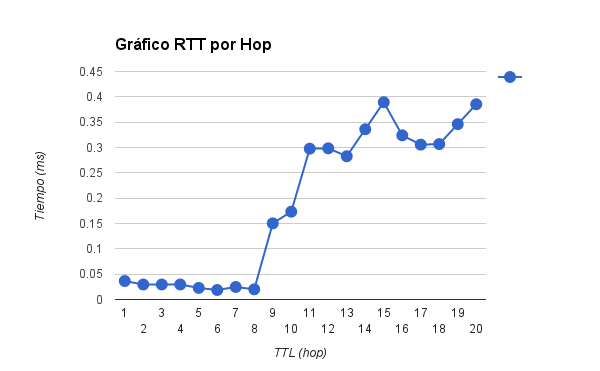
\includegraphics[width=0.7\textwidth]{img_analisis1/rtt_hop.png}
     %\label{fig:ICMPlista} 
	%\end{center} 
    
\end{figure}
\vspace{0.25cm}

%Promedio Delta RTT: 0.00588932037354, 0.223511198044, -0.0304053096771, -0.0112577915192, 0.0367794513702, 0.107529531662, -0.120579014962, 0.0107178688049, 0.107933545113, -0.0993495464325, 0.0167979955673, -0.0487000465393, 0.064146566391, 0.0933417320251, 0.0240439891815, -0.0125254392624, 0.0359566926956, -0.0348659515381, 0.0918450593948, -4.58002090454e-05, -0.00115667533875, 0.00671604824066, 0.0508928060532, -0.0580342292786, 0.00854189395905, 0.00741848945618, -0.143095983322, 0.102489104051\newline
\begin{figure}[h]
	%\begin{center}
    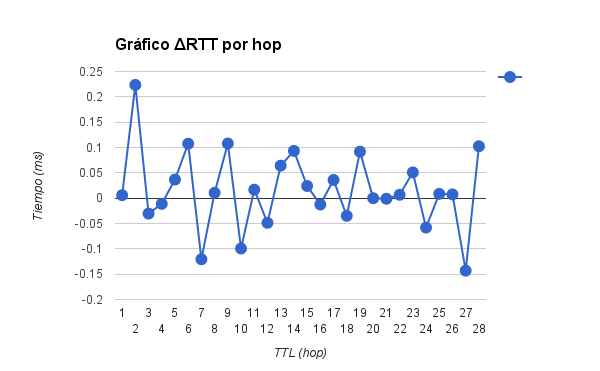
\includegraphics[width=0.7\textwidth]{img_analisis1/delta_rtt_hop.png}
     %\label{fig:ICMPlista} 
	%\end{center} 
    
\end{figure}
\vspace{0.25cm}

%Desvio Estandar Delta RTT: 0.00165442878817, 0.126023742282, 0.071172659274, 0.0745178056825, 0.1866931839, 0.180733182681, 0.0518781646894, 0.065719884364, 0.227576463877, 0.177889865429, 0.0311607993988, 0.0706603578755, 0.147728183499, 0.0762432009451, 0.0966932498659, 0.11828018604, 0.0873092181674, 0.0842616491826, 0.0484700197953, 0.112708845656, 0.0881211770851, 0.0889849976974, 0.0825379976568, 0.0601178559323, 0.0414772504639, 0.0872692906756, 0.0765956277221, 0.0546049405093\newline
\begin{figure}[h]
	%\begin{center}
    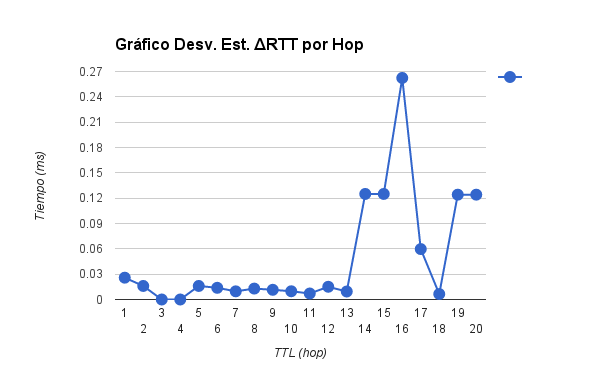
\includegraphics[width=0.7\textwidth]{img_analisis1/ds_delta_rtt_hop.png}
     %\label{fig:ICMPlista} 
	%\end{center} 
    
\end{figure}
\vspace{0.25cm}

De la muestra obtuvimos una distribuci\'on Normal, y los siguientes enlaces submarinos: nodo 2, nodo 5.\newline

Gr\'afico de mapa marcando puntos claves de la ruta:

\subsubsection{Conclusi\'on}
Explicaci\'on de los resultados obtenidos.